\begin{figure}[ht]
\centering
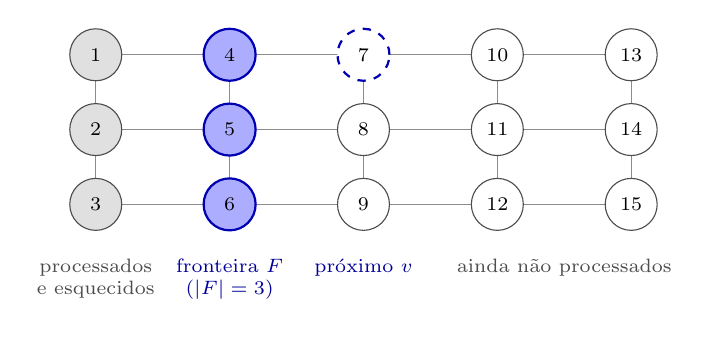
\begin{tikzpicture}[x=1.7cm,y=-0.95cm,
  vtx/.style={circle,draw=black!70,minimum size=0.66cm,inner sep=0pt,font=\scriptsize},
  proc/.style={vtx,fill=black!12},
  fron/.style={vtx,fill=blue!32,draw=blue!70!black,thick},
  prox/.style={vtx,fill=white,draw=blue!70!black,thick,dashed},
  nao/.style={vtx,fill=white},
  aresta/.style={draw=black!45}]
  \foreach \c in {1,...,5}{\foreach \r in {1,2,3}{
    \pgfmathtruncatemacro{\id}{(\c-1)*3+\r}
    \coordinate (p\c\r) at (\c,\r);
  }}
  \foreach \c in {1,...,5}{\foreach \r in {1,2,3}{
    \pgfmathtruncatemacro{\cc}{\c+1}\pgfmathtruncatemacro{\rr}{\r+1}
    \ifnum\c<5 \draw[aresta] (p\c\r) -- (p\cc\r); \fi
    \ifnum\r<3 \draw[aresta] (p\c\r) -- (p\c\rr); \fi
  }}
  \foreach \c/\sty in {1/proc,2/fron,3/nao,4/nao,5/nao}{\foreach \r in {1,2,3}{
    \pgfmathtruncatemacro{\id}{(\c-1)*3+\r}
    \ifnum\c=3\ifnum\r=1 \node[prox] at (p\c\r) {\id}; \else \node[nao] at (p\c\r) {\id}; \fi
    \else \node[\sty] at (p\c\r) {\id}; \fi
  }}
  \node[anchor=north,align=center,font=\scriptsize,text=black!70] at (1,3.6) {processados\\e esquecidos};
  \node[anchor=north,align=center,font=\scriptsize,text=blue!60!black] at (2,3.6) {fronteira $F$\\($|F|=3$)};
  \node[anchor=north,align=center,font=\scriptsize,text=blue!60!black] at (3,3.6) {próximo $v$};
  \node[anchor=north,align=center,font=\scriptsize,text=black!70] at (4.5,3.6) {ainda não processados};
\end{tikzpicture}
\caption{Percurso da programação dinâmica em uma grade $3\times5$ numerada por colunas. Os vértices 1 a 3 já saíram da fronteira (todos os seus vizinhos foram processados); os vértices 4 a 6 formam a fronteira $F$, porque cada um ainda tem vizinho na coluna seguinte. Ao inserir o vértice 7, a tabela tem $2^{|F|+1}=16$ entradas.}\label{fig:fronteira}
\end{figure}
